\documentclass{article}
\usepackage{v-test-paper}
\usepackage{pgfplots}
\renewcommand{\frac}{\dfrac}
% \renewcommand{\ans}{}

\title{\textsc{NAIET Test Paper\\(Maths)}}
\date{}
\begin{document}
\maketitle
\begin{enumerate}
    \item If \(  \ln(7) = x \) then the value of  \( \ln \left( \dfrac{1}{7e} \right) \) is
        \begin{tasks}(4)
        	\task \( -x + 1 \)
        	\task \( x - 1 \)
        	\task \( x + 1 \)
        	\task \( -x - 1 \)\ans
        \end{tasks}
    \item Find the quadratic equation whose graph is
        \begin{center}
            
\begin{tikzpicture}[scale=0.8]
              \tzaxes(-2, -1)(5, 4){$x$}{$y$}
              \tzfn{0.5*(\x-1)*(\x-3)}[-1:4.5]
              \tzticks{1/1, 3/3}
            \end{tikzpicture}
        \end{center}
        \begin{tasks}(4)
        	\task \( y = x^2 - 4x + 3 \)\ans
        	\task \( y = -x^2 + 4x + 3 \)
        	\task \( y = -x^2 - 4x - 3 \)
        	\task \( y = x^2 + 4x - 3 \)
        \end{tasks}
    \item If \( \cot(x) = 4 \) then what is value of \( \dfrac{\cos(x) - \sin(x)}{\cos(x) + 2 \sin(x)} \) is
        \begin{tasks}(4)
        	\task \( \dfrac{1}{3} \)
        	\task \( \dfrac{1}{4} \)
        	\task \( \dfrac{1}{2} \)\ans
        	\task \( 0 \)
        \end{tasks}
    \item The tops of two poles of height \( 20\sqrt{2} \) m and \( 14 \sqrt{2}\) m are connected by a wire. If the wire makes an angle \( 45^\circ \) with horizontal then length of wire in meter is
        \begin{tasks}(4)
        	\task \( 13 \)
        	\task \( 12 \)\ans
        	\task \( 40 \)
        	\task \( 28 \)
        \end{tasks}
    \item Let \( f(x) = \begin{cases}
    			3x + a & \text{if} \ x \leq 2 \\
    			x - 2 & \text{if} \ x > 2 \\
    		   \end{cases} \), what is the value of \( 'a' \) if \( \lim\limits_{x \to 2} f(x) \) exists
        \begin{tasks}(4)
        	\task \( -3 \)
        	\task \( -4 \)
        	\task \( -5 \)
        	\task \( -6 \)\ans
        \end{tasks}
    \item The figure shows the graph of \( y = 2^x \), \( y = 3^{-x} \) and \( y = -\ln(x) \). Match the following
    % The task for matching is not provided, thus cannot be translated to LaTeX tasks
    \begin{center}
        \begin{tikzpicture}
            \tzaxes(-4, -2)(4, 4){$x$}{$y$}
            \tzfn{2^\x}[-4:2]{$B$}[r]
            \tzfn{-ln(\x)}[0.05:3]{$C$}[r]
            \tzfn{3^(-\x)}[-1.25:4]
            \tznode(-1.5, 3){$A$}
            \tzticks{1/1}{1/1}
            \end{tikzpicture}
    \end{center}
    \begin{tasks}(2)
        \task \( A \rightarrow 2^x \quad B \rightarrow 3^{-x} \quad C \rightarrow -\ln x \)
        \task \( A \rightarrow 3^{-x} \quad B \rightarrow 2^x \quad C \rightarrow -\ln x \)\ans
        \task \( A \rightarrow -\ln(x) \quad B \rightarrow 2^x \quad C \rightarrow 3^{-x} \)
        \task \( A \rightarrow 2^x \quad B \rightarrow -\ln x \quad C \rightarrow 3^{-x} \)
      \end{tasks}

    \item In the following fig. find the coordinates of $M$.
    \begin{center}
        \begin{tikzpicture}
            \tzline(-3, 0)(3, 0){$y=2x+3$}[r]
            \tzline(0, 0)(0, 2){$(1, 2)$}[r]
            \tzcoor*(0, 2)(A)
            \tzcoor*(0, 0)(M){$M$}[b]
            \tzrectangle(0, 0)(0.25, 0.25)
        \end{tikzpicture}
    \end{center}
        \begin{tasks}(4)
            	\task $\left(-\frac{1}{5}, \frac{13}{5}\right)$\ans
            	\task $\left(\frac{13}{5}, -\frac{1}{5}\right)$
            	\task $\left(-\frac{13}{5}, \frac{1}{5}\right)$
            	\task $\left(\frac{1}{5}, -\frac{13}{5}\right)$
        \end{tasks}
    \item The line $x+y=2$, $x$-axis and $y$-axis make a triangle, what is the area of this triangle?
        \begin{tasks}(4)
            	\task $1$
            	\task $3$
            	\task $2$\ans
            	\task $4$
        \end{tasks}
    \item In fig. $O$ is center of circle and $OABC$ is rectangle and $OA=3$cm, $AD=2$cm then length of $AC$ is
    \begin{center}
        
\begin{tikzpicture}
            \tzcoor*(0, 0)(O){$O$}[b]
            \def\R{2}
            \tzcircle(O)(\R)
            \tzline(O)(\R, 0){$D$}[r]
            \tzline+(60:\R)(0, -\R*sin{60}){$A$}[b]
            \tzline+(60:\R)(-\R*cos{60}, 0){$C$}[l]
            \tzline(O)(90:\R)
            \tznode(60:\R){$B$}[ar]
            \tzline[dashed](\R*cos{60}, 0)(0, \R*sin{60})
        \end{tikzpicture}
    \end{center}
        \begin{tasks}(4)
            	\task $5$cm\ans
            	\task $3$cm
            	\task $2$cm
            	\task $10$cm
        \end{tasks}
    \item Define $|x| = \begin{cases} 
          x & \text{if } x\geq 0 \\
          -x & \text{if } x<0 
       \end{cases}$, Then which of the following statement is true?
        \begin{tasks}(2)
            	\task $|x| = x^2$ for $x\in \mathbb{R}$
            	\task $|x| \neq x^2$ for $x\in \mathbb{R}$
            	\task $\sqrt{x^2} = x$ for $x\in \mathbb{R}$
            	\task $|x| = x$ has infinitely many solutions.\ans
        \end{tasks}
    \item Find the area of shaded region.
    \begin{center}
        
\begin{tikzpicture}[scale=1.5, xscale=1.2]
            \tzaxes(-0.5, -0.5)(2.5, 2.5){$x$}{$y$}
            \tzlines[pattern=north east lines](0, 0)(1, 1)(0, 2)(0, 0);
            \tzcoor*(1, 1)(A){$(1, 1)$}[r]
            \tznode(0.5, 0.5){$y=x$}[r]
            \tznode(0.5, 1.5){$y=2-x$}[ar]
            \tznode(0, 2){$(0, 2)$}[r]
            \tzticks{0/0, 1/1}{1/1, 2/2}
        \end{tikzpicture}
    \end{center}
        \begin{tasks}(4)
            	\task $1$\ans
            	\task $2$
            	\task $3$
            	\task $4$
        \end{tasks}
    \item In right angle triangle $\triangle ABC$, $\angle C=90^\circ$, $AC = 2\sqrt{2}$ and $AB = BC$ then $\cos(C) =$
        \begin{tasks}(4)
            	\task $\sqrt{2}$
            	\task $\frac{1}{\sqrt{2}}$\ans
            	\task $\frac{1}{2}$
            	\task $1$
        \end{tasks}
    \item Let $f(x) = \frac{x^2-4}{x^2+x-6}$ and it is continues at $x=2$ then which of following is true?
        \begin{tasks}(4)
            	\task $f(2) = 1$
            	\task $f(2) = \frac{5}{4}$
            	\task $f(2) = \frac{4}{5}$\ans
            	\task $f(2) = 0$
        \end{tasks}
    \item Given that $f(2) = 1, f'(2) = -3, g(2) = 4, g'(2) = 0$ then $\frac{d}{dx}\left(\frac{f(x)}{g(x)}\right)$ at $x=2$ is
        \begin{tasks}(4)
            	\task $-\frac{3}{4}$\ans
            	\task $\frac{3}{4}$
            	\task $\frac{4}{3}$
            	\task $-\frac{4}{3}$
        \end{tasks}
    \item If $\int \cos^7(x) \sin(x) dx = A \cos^8(x) + C$ then value of $A$ is
        \begin{tasks}(4)
            	\task $\frac{1}{8}$
            	\task $-\frac{1}{8}$\ans
            	\task $8$
            	\task $-8$
        \end{tasks}

    \item Let \( A = \begin{pmatrix} 1 & 2 & 3 \\ -3 & 0 & 4 \\ 2 & 5 & 0 \end{pmatrix} \) then sum of elements of \( Ae_1 \) is where \( e_1 = \begin{pmatrix} 1 \\ 0 \\ 0 \end{pmatrix} \)
        \begin{tasks}(4)
            \task \( 6 \)
            \task \( 1 \)
            \task \( 7 \)
            \task \( 0 \)\ans
        \end{tasks}
    \item \(\int_{-1}^{1} x^2 |x| dx \) is equal to
        \begin{tasks}(4)
            \task \( \frac{1}{3} \)
            \task \( \frac{1}{2} \)\ans
            \task \( \frac{1}{4} \)
            \task \( 2 \)
        \end{tasks}
    \item The function \( f(x) = x^2 + 8, x \in \mathbb{R} \) then which is correct?
        \begin{tasks}(2)
            \task it is increasing.
            \task it is decreasing.
            \task it is neither increasing nor decreasing.\ans
            \task maximum value of \( f \) exists.
        \end{tasks}
    \item Let \( A \) be a \(3 \times 3\) matrix such that \( |A| = 64 \) then value of \( \left|\frac{1}{4}A\right| \) is equal to (where \( |A| = \text{det}(A) \))
        \begin{tasks}(4)
            \task \( 2 \)
            \task \( 1 \)\ans
            \task \( 9 \)
            \task \( 16 \)
        \end{tasks}
    \item The value of \( \lim\limits_{x \to \infty} \frac{x^2 + 4x + 1}{5x^2 + 3x + 2} \) is
        \begin{tasks}(4)
            \task \( \frac{1}{2} \)
            \task \( 5 \)
            \task \( \frac{2}{5} \)
            \task \( \frac{1}{5} \)\ans
        \end{tasks}
\end{enumerate}

\begin{center}
\texttt{Answer Key}
\begin{multicols}{5}
\begin{enumerate}
\item (b)
\item (a)
\item (b)
\item (c)
\item (d)
\item (a)
\item (b)
\item (c)
\item (a)
\item (a)
\item (b)
\item (a)
\item (b)
\item (a)
\end{enumerate}
\end{multicols}
\end{center}

\end{document}